% For generating graphs, mostly waveforms

\documentclass
[varwidth, convert={density=1024, size=1024x768, outext=.png}]
{standalone}

%\documentclass{article}

\usepackage{libertine}

\usepackage[libertine]{newtxmath}

\usepackage{tikz}

\begin{document}



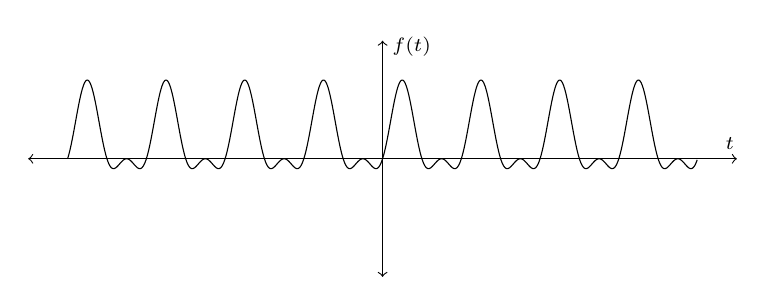
\begin{tikzpicture}

	\tikzstyle{every node}=[font=\scriptsize]

	% x axis
	\draw [<->]
	      (-4.5, 0) 
	   -- (4.5, 0) node [pos=0.99, above] {$t$};

	% y axis
	\draw [<->] 
	      (0, -1.5) 
	   -- (0,  1.5) node [pos=0.975, right] {$f(t)$};

    \draw [domain=-4:4, samples=1000]
          plot(\x, { (0.5 + (0.5 * sin(2 * pi * \x r))) * sin(2 * pi * \x r) });

\end{tikzpicture}


\iffalse

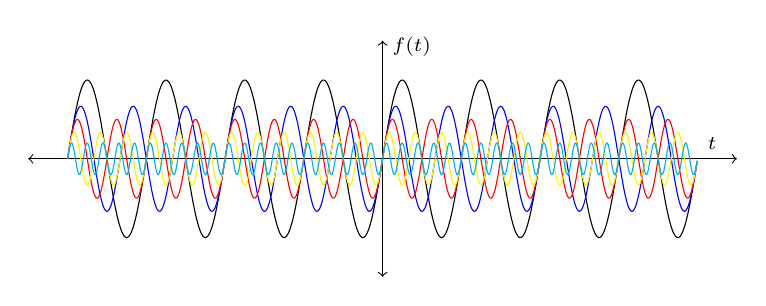
\begin{tikzpicture}[font=\scriptsize]

	% x axis
	\draw [<->]
	      (-4.5, 0) 
	   -- (4.5, 0) node [pos=0.965, above] {$t$};

	% y axis
	\draw [<->] 
	      (0, -1.5) 
	   -- (0,  1.5) node [pos=0.975, right] {$f(t)$};

    \draw [domain=-4:4, samples=1000]
          plot(\x, {1/1 * sin(2 * pi * \x r)});

    \draw [domain=-4:4, samples=1000, blue]
          plot(\x, {2/3 * sin(3 * pi * \x r)});

    \draw [domain=-4:4, samples=1000, red]
          plot(\x, {1/2 * sin(4 * pi * \x r)});

    \draw [domain=-4:4, samples=1000, yellow]
          plot(\x, {1/3 * sin(6 * pi * \x r)});

    \draw [domain=-4:4, samples=1000, cyan]
          plot(\x, {1/5 * sin(10 * pi * \x r)});      

\end{tikzpicture}

\par $$\Downarrow$$ \par
\fi

\iffalse

\begin{tikzpicture}
	% Just for scaling the "graph"
	\draw (0, -1.5) (0, 1.5);

	% The arrow
	\draw (0, 0) node {$\,$\hspace{0.5cm}$\Rightarrow$\hspace{0.5cm}$\,$};
\end{tikzpicture}

\fi

\iffalse
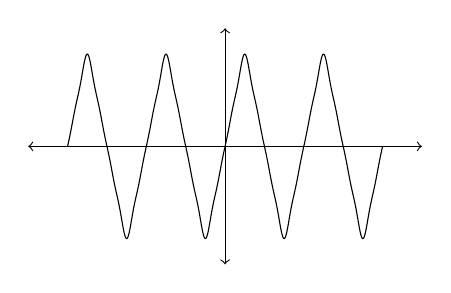
\begin{tikzpicture}

	\tikzstyle{every node}=[font=\scriptsize]

	% x axis
	\draw [<->]
	      (-2.5, 0) 
	   -- (2.5, 0);% node [pos=0.965, above] {$t$};

	% y axis
	\draw [<->] 
	      (0, -1.5) 
	   -- (0,  1.5);% node [pos=0.975, right] {$f(t)$};

    \draw [domain=-2:2, samples=1000]
          plot(\x, {
          				1 * 
          				(
	          				1/1 * (sin(2 * pi * \x r)   +
	                    	-1/9 * sin(6 * pi * \x r))   +
	                    	1/25 * sin(10 * pi * \x r)) + 
	                    	-1/49 * sin(14 * pi * \x r))
                    	)
                    });

\end{tikzpicture}
\fi

\iffalse

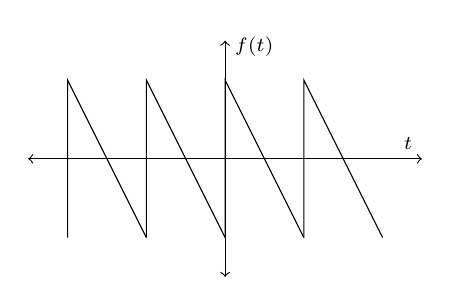
\begin{tikzpicture}

	\tikzstyle{every node}=[font=\scriptsize]

	% x axis
	\draw [<->]
	      (-2.5, 0) 
	   -- (2.5, 0) node [pos=0.965, above] {$t$};

	% y axis
	\draw [<->] 
	      (0, -1.5) 
	   -- (0,  1.5) node [pos=0.975, right] {$f(t)$};

    \foreach \i in {-2, -1, 0, 1} 
    {
    	\draw (\i, -1) -- (\i, 1) -- (\i + 1, -1);
    }

\end{tikzpicture}

\fi

\end{document}